\subsection{Paquete 4: Comunidad de convivencia y espacio del hogar}

    El paquete estructura la convivencia tras confirmarse el arrendamiento. Permite unir nuevos compañeros mediante códigos dinámicos de un solo uso, personalizar avatares, registrar eventos en un muro de actividad inmutable y tramitar expulsiones o bajas voluntarias siempre que no existan deudas abiertas. La figura \ref{fig:dcu_convivencia} modela los once casos de uso que componen este espacio compartido (CU39 a CU49).

\begin{figure}[H]
    \centering
    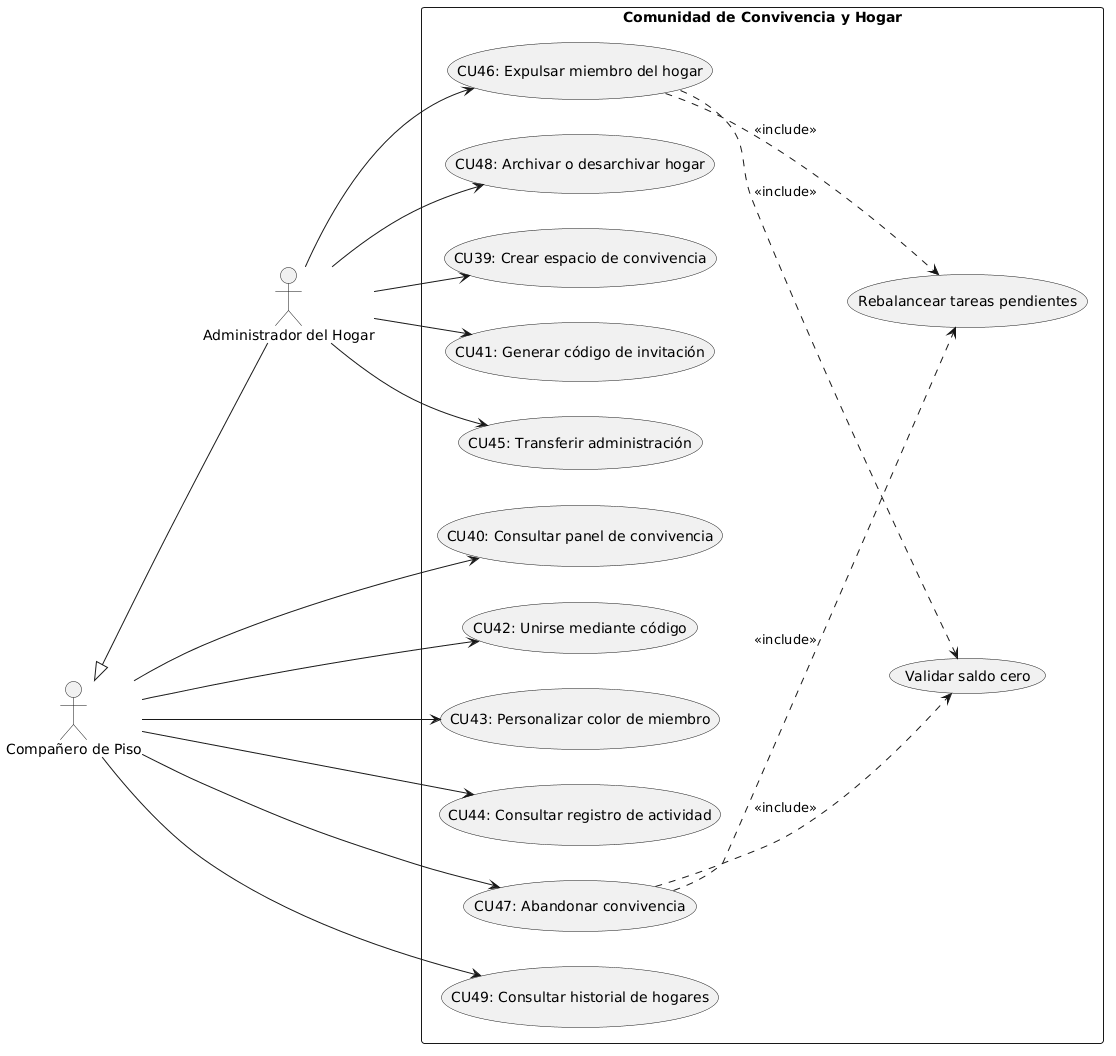
\includegraphics[width=0.85\textwidth]{AnalisisFuncional/img/dcu_convivencia.png}
    \caption{Diagrama de casos de uso de comunidad de convivencia y hogar}
    \label{fig:dcu_convivencia}
\end{figure}

    Las siguientes especificaciones describen los casos de uso asociados al hogar (CU39 a CU49):

\begin{table}[H]
\centering
\begin{tabular}{|p{3.2cm}|p{11.3cm}|}
\hline
\textbf{Caso de Uso} & \textbf{CU39: Crear espacio de convivencia} \\ \hline
\textbf{Actores} & Administrador del Hogar \\ \hline
\textbf{Descripción} & Da de alta un nuevo grupo de piso asignando nombre, dirección y reglas básicas \\ \hline
\textbf{Precondiciones} & Estar autenticado y no pertenecer a otro hogar en calidad de administrador simultáneo \\ \hline
\textbf{Flujo básico} & 
1. El usuario accede al formulario de creación de comunidad e introduce los datos del piso. \newline
2. El sistema valida la información e inicializa el espacio de convivencia. \newline
3. El backend otorga al creador el rol de administrador del hogar. \newline
4. El sistema redirige al panel principal del nuevo hogar. \\ \hline
\end{tabular}
\caption{Especificación del caso de uso CU39}
\label{tab:cu39}
\end{table}

\begin{table}[H]
\centering
\begin{tabular}{|p{3.2cm}|p{11.3cm}|}
\hline
\textbf{Caso de Uso} & \textbf{CU40: Consultar panel y detalle de convivencia} \\ \hline
\textbf{Actores} & Compañero de Piso \\ \hline
\textbf{Descripción} & Muestra la vista global del piso con la lista de miembros, balances rápidos y avisos \\ \hline
\textbf{Precondiciones} & Pertenecer activamente al hogar consultado \\ \hline
\textbf{Flujo básico} & 
1. El usuario accede a la sección de inicio del piso en la interfaz. \newline
2. El sistema recupera los datos de los integrantes, sus roles y estados asignados. \newline
3. La interfaz renderiza el resumen consolidado de convivencia y accesos a módulos. \\ \hline
\end{tabular}
\caption{Especificación del caso de uso CU40}
\label{tab:cu40}
\end{table}

\begin{table}[H]
\centering
\begin{tabular}{|p{3.2cm}|p{11.3cm}|}
\hline
\textbf{Caso de Uso} & \textbf{CU41: Generar o regenerar código de invitación} \\ \hline
\textbf{Actores} & Administrador del Hogar \\ \hline
\textbf{Descripción} & Crea o renueva una clave alfanumérica única para la incorporación de compañeros \\ \hline
\textbf{Precondiciones} & Poseer el rol de administrador en el hogar activo \\ \hline
\textbf{Flujo básico} & 
1. El administrador accede a la sección de invitaciones del piso. \newline
2. El administrador solicita la emisión o sustitución del código de acceso. \newline
3. El backend genera una cadena alfanumérica unívoca e invalida la anterior. \newline
4. La interfaz presenta la clave lista para ser compartida por canales externos. \\ \hline
\end{tabular}
\caption{Especificación del caso de uso CU41}
\label{tab:cu41}
\end{table}

\begin{table}[H]
\centering
\begin{tabular}{|p{3.2cm}|p{11.3cm}|}
\hline
\textbf{Caso de Uso} & \textbf{CU42: Unirse a un hogar mediante código} \\ \hline
\textbf{Actores} & Compañero de Piso \\ \hline
\textbf{Descripción} & Permite a un usuario vincularse a un piso introduciendo la clave de invitación \\ \hline
\textbf{Precondiciones} & Estar autenticado en el sistema y disponer de un código de invitación válido \\ \hline
\textbf{Flujo básico} & 
1. El usuario introduce el código alfanumérico en la pantalla de bienvenida o unirse. \newline
2. El backend verifica la autenticidad y vigencia de la clave introducida. \newline
3. El sistema añade al usuario como compañero activo del hogar. \newline
4. El sistema notifica la incorporación en el muro general de actividad. \\ \hline
\end{tabular}
\caption{Especificación del caso de uso CU42}
\label{tab:cu42}
\end{table}

\begin{table}[H]
\centering
\begin{tabular}{|p{3.2cm}|p{11.3cm}|}
\hline
\textbf{Caso de Uso} & \textbf{CU43: Personalizar color de identificación} \\ \hline
\textbf{Actores} & Compañero de Piso \\ \hline
\textbf{Descripción} & Configura la tonalidad cromática asignada al usuario para calendarios y balances \\ \hline
\textbf{Precondiciones} & Ser miembro activo del piso \\ \hline
\textbf{Flujo básico} & 
1. El compañero abre el selector de color en la configuración de su tarjeta de miembro. \newline
2. El compañero selecciona una tonalidad disponible en la paleta del hogar. \newline
3. El backend persiste la preferencia cromática asociada a la membresía. \newline
4. La interfaz actualiza los distintivos del usuario en tareas y cuadrantes. \\ \hline
\end{tabular}
\caption{Especificación del caso de uso CU43}
\label{tab:cu43}
\end{table}

\begin{table}[H]
\centering
\begin{tabular}{|p{3.2cm}|p{11.3cm}|}
\hline
\textbf{Caso de Uso} & \textbf{CU44: Consultar registro cronológico de actividad} \\ \hline
\textbf{Actores} & Compañero de Piso \\ \hline
\textbf{Descripción} & Despliega el histórico auditable de sucesos relevantes acontecidos en el hogar \\ \hline
\textbf{Precondiciones} & Pertenecer al hogar correspondiente \\ \hline
\textbf{Flujo básico} & 
1. El compañero accede a la pestaña de actividad reciente del piso. \newline
2. El sistema recupera los registros ordenados cronológicamente de forma descendente. \newline
3. La interfaz visualiza eventos de gastos, liquidaciones, tareas y cambios de miembros. \\ \hline
\end{tabular}
\caption{Especificación del caso de uso CU44}
\label{tab:cu44}
\end{table}

\begin{table}[H]
\centering
\begin{tabular}{|p{3.2cm}|p{11.3cm}|}
\hline
\textbf{Caso de Uso} & \textbf{CU45: Transferir privilegios de administrador} \\ \hline
\textbf{Actores} & Administrador del Hogar \\ \hline
\textbf{Descripción} & Traspasa la condición de administrador del espacio a otro compañero de piso \\ \hline
\textbf{Precondiciones} & Ser el administrador vigente y seleccionar un miembro activo diferente \\ \hline
\textbf{Flujo básico} & 
1. El administrador elige a un compañero y pulsa la opción de cesión de privilegios. \newline
2. El sistema solicita confirmación formal para prevenir transferencias involuntarias. \newline
3. El backend reasigna los roles de membresía en la base de datos de manera atómica. \newline
4. El sistema actualiza los permisos de acceso y emite un evento en el feed del hogar. \\ \hline
\end{tabular}
\caption{Especificación del caso de uso CU45}
\label{tab:cu45}
\end{table}

\begin{table}[H]
\centering
\begin{tabular}{|p{3.2cm}|p{11.3cm}|}
\hline
\textbf{Caso de Uso} & \textbf{CU46: Expulsar miembro del hogar} \\ \hline
\textbf{Actores} & Administrador del Hogar \\ \hline
\textbf{Descripción} & Da de baja forzosa a un integrante del piso tras validar la liquidación de sus saldos \\ \hline
\textbf{Precondiciones} & Que el integrante a expulsar no ostente deudas ni créditos pendientes \\ \hline
\textbf{Flujo básico} & 
1. El administrador selecciona la acción de expulsión sobre el integrante. \newline
2. El sistema verifica obligatoriamente que el saldo neto del integrante sea cero. \newline
3. El sistema ejecuta el rebalanceo automático de las tareas domésticas pendientes. \newline
4. El backend conmuta el estado de la membresía a inactiva y revoca sus accesos al piso. \\ \hline
\end{tabular}
\caption{Especificación del caso de uso CU46}
\label{tab:cu46}
\end{table}

\begin{table}[H]
\centering
\begin{tabular}{|p{3.2cm}|p{11.3cm}|}
\hline
\textbf{Caso de Uso} & \textbf{CU47: Abandonar convivencia} \\ \hline
\textbf{Actores} & Compañero de Piso \\ \hline
\textbf{Descripción} & Tramita la baja voluntaria del usuario del espacio de convivencia \\ \hline
\textbf{Precondiciones} & Mantener un balance financiero equilibrado en cero y no ser el único administrador \\ \hline
\textbf{Flujo básico} & 
1. El compañero selecciona la opción de abandonar el hogar desde los ajustes. \newline
2. El sistema comprueba de forma obligatoria que su balance contable sea exactamente cero. \newline
3. El sistema reasigna de manera automática las tareas domésticas que tenía asignadas. \newline
4. El backend desvincula al usuario y archiva su registro histórico en el hogar. \\ \hline
\end{tabular}
\caption{Especificación del caso de uso CU47}
\label{tab:cu47}
\end{table}

\begin{table}[H]
\centering
\begin{tabular}{|p{3.2cm}|p{11.3cm}|}
\hline
\textbf{Caso de Uso} & \textbf{CU48: Archivar o desarchivar vista de hogar} \\ \hline
\textbf{Actores} & Administrador del Hogar \\ \hline
\textbf{Descripción} & Oculta la visualización activa de un piso concluido sin eliminar sus datos históricos \\ \hline
\textbf{Precondiciones} & Que no existan estancias en curso ni deudas monetarias abiertas \\ \hline
\textbf{Flujo básico} & 
1. El administrador activa la conmutación de archivado en la configuración del piso. \newline
2. El sistema comprueba el cierre satisfactorio de todos los compromisos comunes. \newline
3. El backend traslada el hogar al archivo histórico de los participantes. \\ \hline
\end{tabular}
\caption{Especificación del caso de uso CU48}
\label{tab:cu48}
\end{table}

\begin{table}[H]
\centering
\begin{tabular}{|p{3.2cm}|p{11.3cm}|}
\hline
\textbf{Caso de Uso} & \textbf{CU49: Consultar historial de hogares pasados} \\ \hline
\textbf{Actores} & Administrador del Hogar, Compañero de Piso \\ \hline
\textbf{Descripción} & Permite revisar datos y registros de pisos en los que se participó anteriormente \\ \hline
\textbf{Precondiciones} & Haber formado parte de al menos una convivencia finalizada o archivada \\ \hline
\textbf{Flujo básico} & 
1. El usuario accede a la sección de archivos de convivencia en su panel personal. \newline
2. El sistema recupera los expedientes históricos en modo de solo lectura. \newline
3. La interfaz presenta los resúmenes de estancias, compañeros y balances consolidados. \\ \hline
\end{tabular}
\caption{Especificación del caso de uso CU49}
\label{tab:cu49}
\end{table}